% Created 2011-01-05 Ср. 21:05
\documentclass[12pt, russian, oneside, article]{ncc}
\usepackage[utf8]{inputenc}
\usepackage[T1]{fontenc}
\usepackage{fixltx2e}
\usepackage{graphicx}
\usepackage{longtable}
\usepackage{float}
\usepackage{wrapfig}
\usepackage{soul}
\usepackage{textcomp}
\usepackage{marvosym}
\usepackage{wasysym}
\usepackage{latexsym}
\usepackage{amssymb}
\usepackage{hyperref}
\tolerance=1000
\usepackage[math]{pscyr}
\usepackage{indentfirst}
\providecommand{\alert}[1]{\textbf{#1}}
\begin{document}



\title{Квантовая и оптическая электроника}
\author{Максим Захаров}
\date{05 Январь 2011}
\maketitle

\setcounter{tocdepth}{3}
\tableofcontents
\vspace*{1cm}

\href{file:///home/maxim/Documents/Git/lectures/other/KOE_Lectures.pdf}{Скачать в PDF}

\section{Лекция 1}
\label{sec-1}


КОЭ --- новое направление в науке и технике, соединяющее в себе возможности оптики и электроники и появившаяся как отклик на новые потребности человеческой деятельности.

По возможностям превосходит оптику и электронику. Словом КОЭ впервые назвали средства и оборудование, осуществляющее оптическую связь.

В 60 годы, когда появились первые образцы лазеров, позволяющие получать когерентное излучение и давшие возможность проще использовать оптические эффекты, резко возросло число попыток использовать оптику в электронике, а появление методов и способов лазерной голографии открыло возможность получать копии электр. изображений.

В отличие от эл. техники, в которой использовались законы движения заряженных частиц (электронов и дырок в полупроводниках) эти законы использовались для получения, обработки и передачи информации в виде временных рядов.

С появление когерентного оптического излучения законы распространения света были упрощены для реализации и получение, обработка и передача информации уже смогла осуществляться без разложения спектра в виде передачи изображений.

Области применения и перспективы КОЭ. 

Генеалогическое дерево КОЭ.

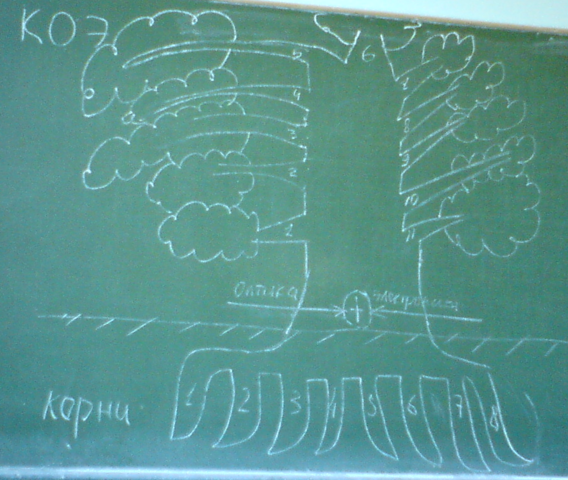
\includegraphics[width=0.5\textwidth]{images/KOE/tree.png}

Корневая система этого дерева расшифровывает свойства излучения и возможности оптоэлектронных систем:
\begin{enumerate}
\item Возможность расширения диапазона частот вплоть до оптической временной частоты.
\item Слабое влияние электромагнитных помех.
\item Бесконтактность получения и обработки информации.
\item Параллельность обработки информации.
\item Когерентность. Временная когерентность --- сама частота временная очень стабильна по девиации частоты.
\item Направленность распространения лазерных пучков. Пространственная когерентность.
\item Монохроматичность характеризуется степенью монохроматичности, которая измеряется в относительных единицах ширины спектральной линии к абсолютному его значению.
\item Фокусируемость. Сфокусированный лазерный пучок в фокальной плоскости фокусирующей системы характер. кружком Эйлера. Это даёт возможность концентрировать энергию лазерного излучения для того, чтобы испарять и твёрдые металлы, включая даже алмазы.
\end{enumerate}

Ветви:
\begin{enumerate}
\item Оптическая связь, которая включает связь по оптическим волокнам, космическая оптическая связь.
\item Промышленные измерения.

\begin{itemize}
\item не разрушающий контроль;
\item точный анализ;
\item галаграфические измерения;
\item сверхскоростные измерения.
\end{itemize}

\item Прочие измерения.

\begin{itemize}
\item измерения загрязнения окружающей среды;
\item определение координат;
\item геологоразведка;
\end{itemize}

\item Сверхскоростная спектроскопия.
\item Спектральный анализ. Включает в себя направления: анализ нелинейных спектров, включая биологический анализ.
\item Фотохимия. Разделение изотопов.
\item Обработка информации.

\begin{itemize}
\item запись на видеодиск;
\item лазерная печать;
\item считывание штриховых кодов;
\item получение трёхмерных изображений.
\item оптическая вычислительная техника, включая средства памяти.
\end{itemize}

\item Медицина.

\begin{itemize}
\item лазерный скальпель;
\item диагностика --- определитель состояния отдельных клеток;
\item тифлотехника;
\end{itemize}

\item Промышленное производство.

\begin{itemize}
\item обработка лазерным излучением;
\item термическая обработка;
\item прецизионная обработка.
\end{itemize}

\item Передача энергии. Посредством лазерных пучков.
\item Производство энергии. Ядерный синтез.
\end{enumerate}
\section{Лекция 2. Оптоэлектронные приборы}
\label{sec-2}


Корневая система:
\begin{enumerate}
\item Неэлектрические эффекты.
\item Фотовольтаический эффект.
\item Фотоэлектрический эффект.
\item Нелинейные оптические эффекты.
\item Магнитооптический эффект.
\item Акустооптический эффект.
\item Электрооптический эффект.
\item Вынужденное излучение и усиление света.
\item Люминесценция.
\end{enumerate}

Ветви:
\begin{enumerate}
\item Фотоприёмники.

\begin{itemize}
\item фотодиод (солнечная батарея);
\item фототранзисторы;
\item лавинный фотодиод;
\item ПЗС элементы (с приборо-зарядовой связью);
\item датчики образа;
\item фотоэлемент, фотоумножитель, пироэлектронные приборы.
\end{itemize}

\item Оптические волноводы.

\begin{itemize}
\item волоконно-оптический волнвод;
\item плёночные волноводы;
\item волноводная линза;
\end{itemize}

\item Оптическая память.

\begin{itemize}
\item устройства на основе фотоплёнки;
\item фотохромные материалы;
\item аморфные полупроводники;
\end{itemize}

\item Функциональные приборы.

\begin{itemize}
\item преобразователь некогерентного излучения в когерентное
\item оптически нестабильный элемент;
\item оптические вентили;
\item оптрон;
\end{itemize}

\item Интеграция.

\begin{itemize}
\item оптические интегральные схемы;
\item оптоэлектронные интегральные схемы;
\end{itemize}

\item Модуляторы света и отклоняющие сканирующие системы.

\begin{itemize}
\item системы зеркал;
\item приборы электромагнитоакустооптические;
\item инжекционные излучатели;
\end{itemize}

\item Дисплеи.

\begin{itemize}
\item светодиодные;
\item электролюминесцентные;
\item фосфорисцентные;
\item жидкокристаллические;
\item электрохромные.
\end{itemize}

\end{enumerate}

\end{document}
